\section{性能评测}
本节将给出若干微基准测试，用以说明GFS架构和实现中固有的瓶颈；
同时也会展示Google正在使用的真实集群的一些数据。

\subsection{微基准测试}
我们在一个由1个master、2个master replica、16个chunkserver和16个客户端组成的GFS
集群上测量性能。请注意，这一配置是为便于测试而搭建的。典型集群拥有数百个chunkserver和数百个客户端。

所有机器均配置双1.4GHz的PIII处理器、2GB内存、两块80GB、5400转/分的磁盘，以及一条连
接到HP2524交换机的100Mbps全双工以太网链路。19台GFS服务器机器全部连接到一台交换机，
16台客户端机器全部连接到另一台交换机。这两台交换机之间通过一条1Gbps链路相连。

\subsubsection{读}
N个客户端同时从文件系统读取数据。每个客户端从一个320GB的文件集合中随机读取一个4MB区域。
该操作重复256次，因此每个客户端最终读取1GB数据。
全部chunkserver的内存总量只有32GB，因此我们预计Linux缓冲区缓存的命中率最多为10\%。
我们的结果应当接近冷缓存条件下的结果。

Figure 3(a)展示了N个客户端的聚合读取速率及其理论上限。该上限取决于
先达到饱和的资源：当两台交换机之间的1Gbps链路饱和时，聚合速率上限为125MB/s；
当单个客户端的100Mbps网络接口饱和时，每个客户端的上限为12.5MB/s。
只有一个客户端读取时，观测到的读取速率为10MB/s，即单客户端上限的80\%。
当有16个读取者时，聚合读取速率达到94MB/s，约为125MB/s链路上限的75\%，即每个客户端约6MB/s。
效率从80\%下降到75\%，是因为随着读取者数量增加，多个读取者同时从同一个chunkserver
读取数据的概率也会增加。

\subsubsection{写}
N个客户端同时向N个不同文件写入数据。每个客户端通过一系列1MB
写入，向一个新文件写入1GB数据。Figure 3(b)展示了聚合写入速率
及其理论上限。该上限稳定在67MB/s，因为每个字节都需要写入16个
chunkserver中的3个，而每个chunkserver的入站连接速率为12.5MB/s。

单个客户端的写入速率为6.3MB/s，约为该上限的一半。造成这一结果的主要原因是我们的网络栈。
它与我们用于向chunk replica推送数据的流水线方案配合得不够好。从一个replica向另一个replica传播数
据时产生的延迟，降低了整体写入速率。

当有16个客户端时，聚合写入速率达到35MB/s(即每个客户端2.2MB/s)，约为理论上限的一半。
与读取情况相同，随着客户端数量增加，多个客户端并发写入同一个chunkserver的可能性也会提高。
此外，16个写入者发生冲突的可能性高于16个读取者，因为每次写入涉及3个不同replica。

写入速度低于我们的预期。在实践中，这并未成为主要问题：尽管它会增加单个客户端所感知的延迟，
但并不会显著影响系统向大量客户端提供的聚合写入带宽。

\subsubsection{Record Append}
Figure 3(c)展示了\textbf{record append}的性能。N个客户端同时向同一个文件追加数据。
性能受存储该文件最后一个chunk的chunkserver网络带宽限制，与客户端数量无关。
单个客户端时速率为6.0MB/s；当客户端数增加到16个时，速率降至4.8MB/s，主要原因是网络拥塞，
以及不同客户端观察到的网络传输速率波动。

我们的应用通常会并发生成多个这样的文件。换言之，N个客户端会同时向M个共享文
件追加数据，其中N和M都达到数十或数百的规模。因此，实验中出现的chunkserver
网络拥塞在实践中并不是显著问题，因为当某个文件对应的chunkserver忙碌时，客户端仍
可以继续写入另一个文件。

\subsection{真实世界的集群}
我们现在考察Google内部正在使用的两个集群，它们可代表其他若干类似集群。
集群A由一百多名工程师定期用于研究与开发。一个典型任务由人工用户发起，
运行时间最长可达数小时。它读取数MB到数TB的数据，对数据进行转换或分析，
并将结果写回集群。集群B主要用于生产数据处理。任务持续时间更长，并且只需偶尔
人工干预，就能持续生成和处理数TB规模的数据集。在两种情况下，一个“任务”都
由分布在多台机器上的许多进程构成，它们会同时读写大量文件。

\subsubsection{存储}
如Table 2的前五项所示，两个集群都拥有数百台chunkserver，提供数十TB的磁盘空间，
且磁盘使用率较高但尚未完全占满。“已用空间”包含所有chunk replica。几乎所有文件都保存了3个
replica。因此，这两个集群分别存储了18TB和52TB的文件数据。

两个集群的文件数量相近，不过集群B中已删除文件所占比例更高，即已被删除或被新
版本替换、但其存储空间尚未回收的文件。由于其中的文件往往更大，它也拥有更多chunk。

\begin{center}
  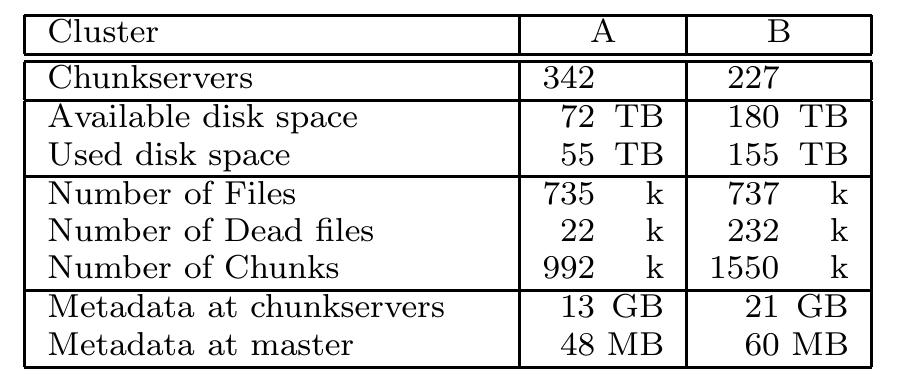
\includegraphics[width=0.95\columnwidth]{figures/original/gfs-table-2-cluster-characteristics.png}
  \refstepcounter{table}\label{tab:gfs-cluster-characteristics}

  {\small\textbf{Table 2.}两个GFS集群的特征}
\end{center}

\subsubsection{元数据}
所有chunkserver合计存储数十GB的元数据，其中大部分是用户数据64KB块的校验和。
chunkserver保存的另一类元数据只有section4.5讨论过的chunk版本号。

master保存的元数据要小得多，只有数十MB，平均每个文件约100字节。这与我们的假设一致：
在实践中，master的内存大小不会限制系统容量。每个文件的大部分元数据是以前缀压缩形式
保存的文件名。其他元数据包括文件所有权和权限、文件到chunk的映射，以及每个chunk的当前版本。
此外，对于每个chunk，我们还保存当前replica位置和用于实现写时复制的引用计数。

每台服务器，无论是chunkserver还是master，都只保存50MB到100MB的元数据。
因此恢复速度很快：服务器只需从磁盘读取这些元数据数秒，便能够响应查询。
不过，master在从所有chunkserver获取chunk位置信息之前，仍会在一段时间内受到限制，
通常为30到60秒。

\begin{figure*}[t]
  \centering
  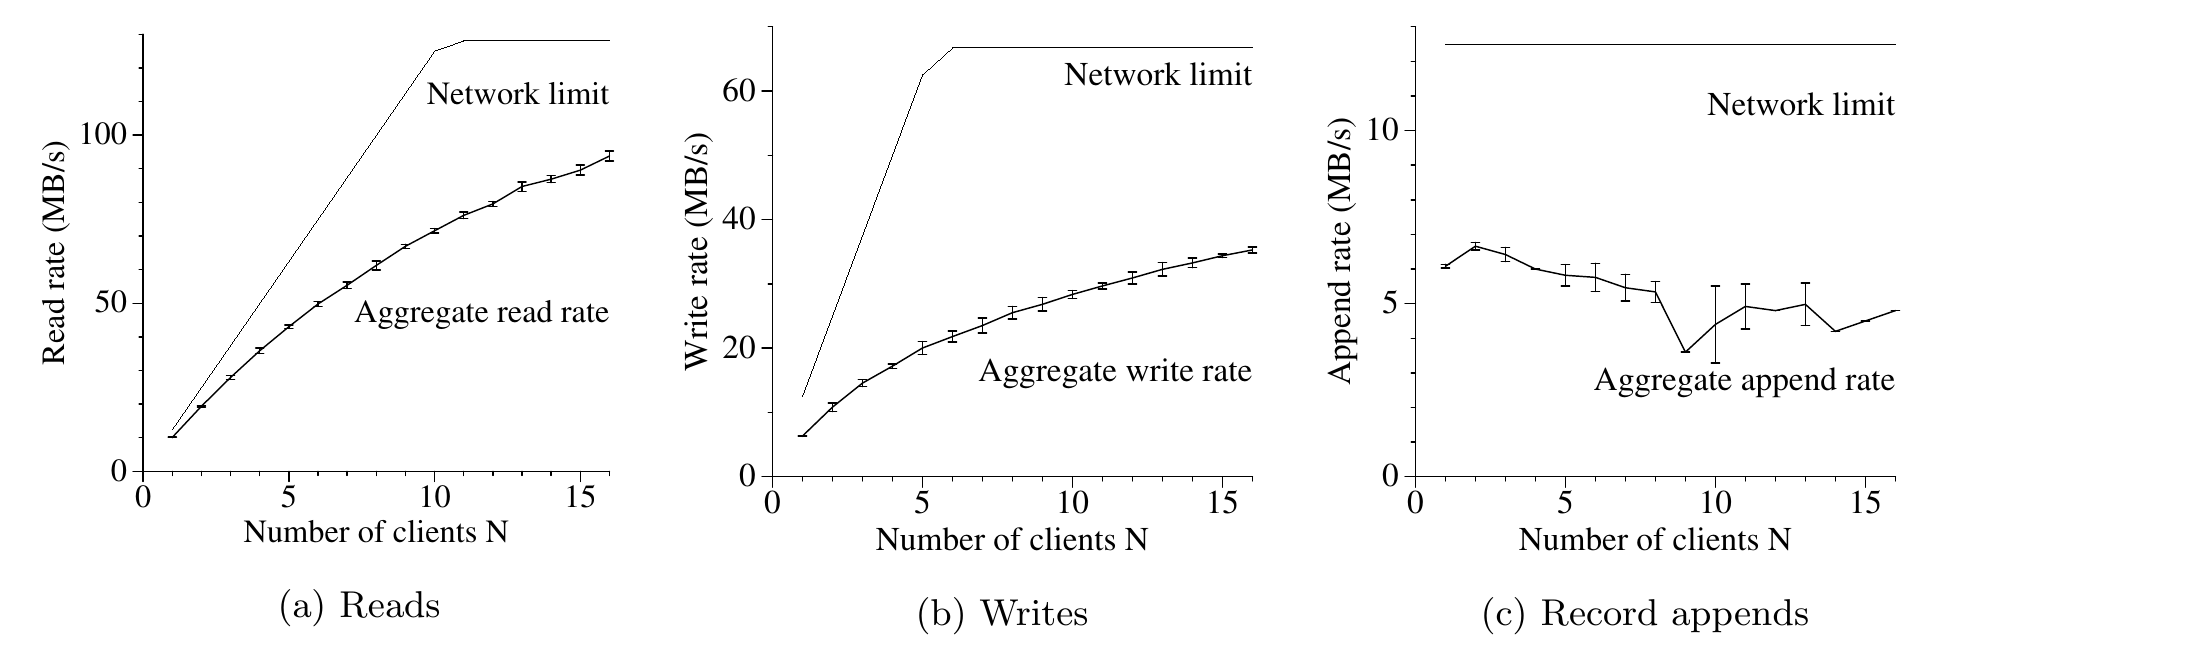
\includegraphics[width=0.96\textwidth]{figures/original/gfs-figure-3-aggregate-throughputs.png}
  \captionsetup{justification=centering}
  \renewcommand{\figurename}{Figure}
  \caption{聚合吞吐量。上方曲线表示网络拓扑带来的理论上限；下方曲线表示测得的吞吐量。误差线表示95\%置信区间；由于测量方差较低，部分误差线难以辨认。}
  \label{fig:gfs-aggregate-throughputs}
\end{figure*}

\subsubsection{读写速率}
Table 3展示了不同时间段内的读写速率。进行这些测量时，两个集群均已运行约一周。
(这些集群不久前曾为升级到新版GFS而重启)

自重启以来，平均写入速率低于30MB/s。我们进行这些测量时，集群B正处于一段写入活动
突发期，产生约100MB/s的数据；由于写入会传播到3个replica，这导致了300MB/s的网络负载。

\begin{center}
  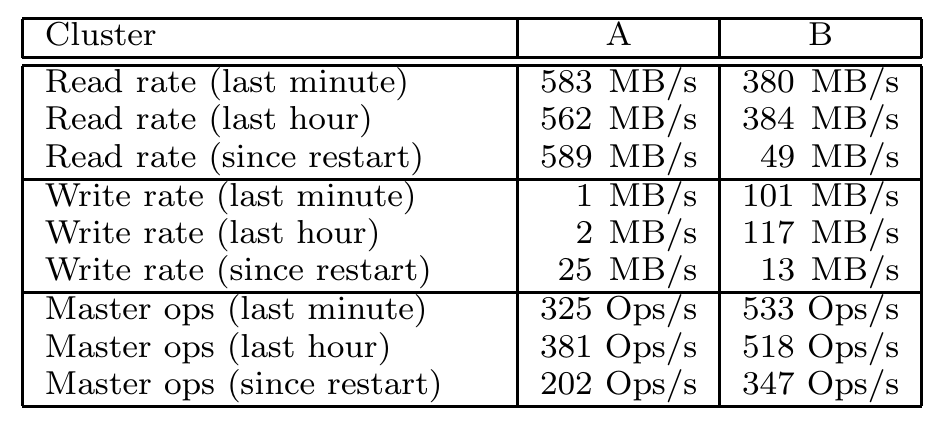
\includegraphics[width=0.95\columnwidth]{figures/original/gfs-table-3-performance-metrics.png}
  \refstepcounter{table}\label{tab:gfs-performance-metrics}

  {\small\textbf{Table 3.}两个GFS集群的性能指标}
\end{center}

读取速率远高于写入速率。正如我们所假设的，整体访问负载中读取操作多于写入操作。
两个集群当时都处于高强度读取活动期间。特别是，集群A在此前一周一直维持580MB/s的读取速率。
它的网络配置可支持750MB/s，因此资源利用较为高效。集群B可支持1300MB/s的峰值读取速率，
但其应用实际只使用了380MB/s。

\subsubsection{master负载}
Table 3还表明，发送给master的操作速率约为每秒200到500次。master可以轻松处理这一速率，
因此不会成为这些访问负载的瓶颈。

在较早版本的GFS中，master偶尔会成为某些访问负载的瓶颈。它大部分时间都在顺序扫
描大型目录(其中包含数十万个文件)，以查找特定文件。此后，我们修改了master的数据结
构，使其能够在命名空间中进行高效的二分查找。现在，它可以轻松支持每秒数千次文件访
问。如有必要，我们还可以在命名空间数据结构之前设置名称查找缓存，进一步提高速度。

\subsubsection{恢复时间}
在一个chunkserver发生故障后，部分chunk会变为replica不足，必须通过克隆恢复其replica数量。
恢复所有这类chunk所需的时间取决于可用资源数量。在一项实验中，我们终止了集群B中
的一台chunkserver。该chunkserver保存约15,000个chunk，共含600GB数据。为限制对运
行中应用的影响，并为调度决策预留余量，我们的默认参数将该集群限制为最多同时执行91个克隆操
作(chunkserver数量的40\%)，且每个克隆操作最多可使用6.25MB/s(50Mbps)的带宽。
所有chunk在23.2分钟内恢复完成，有效复制速率为440MB/s。

在另一项实验中，我们终止了两台chunkserver，每台大约保存16,000个chunk和660GB数据。
这次双重故障使266个chunk只剩下一个replica。我们以更高优先级克隆这266个chunk，
并在2分钟内全部将其恢复到至少2倍replica，使集群能够在不丢失数据的情况下承受另一台
chunkserver故障。


\subsection{访问负载拆解}
本节将详细拆解两个GFS集群上的访问负载。这两个集群与section6.2中的集群具有可比性，
但并不完全相同。集群X用于研究与开发，集群Y用于生产数据处理。

\subsubsection{方法与注意事项}

这些结果只包含由客户端发起的请求，以便反映我们的应用为整个文件系统产生的访问负载。
它们不包括为执行客户端请求而产生的服务器间请求，也不包括内部后台活动，例如转发
写入或负载再平衡。

I/O操作的统计数据基于从GFS服务器记录的实际RPC请求中，以启发式方法重建的信息。
例如，GFS客户端代码可能会将一次读取拆分为多个RPC，以提高并行度；我们据此推断出
原始读取。由于我们的访问模式高度程式化，我们预计任何误差都会落入噪声范围。由应
用显式记录日志或许能提供稍微更准确的数据，但从实际操作角度看，重新编译并重启数千
个正在运行的客户端并不可行，而且从如此多机器收集结果也十分繁琐。

不应过度泛化我们的访问负载。由于Google同时完全控制GFS及其应用，应用往往会针对GFS进
行调优；反过来，GFS也是为这些应用设计的。这种相互影响也可能存在于通用应用之间。

\begin{center}
  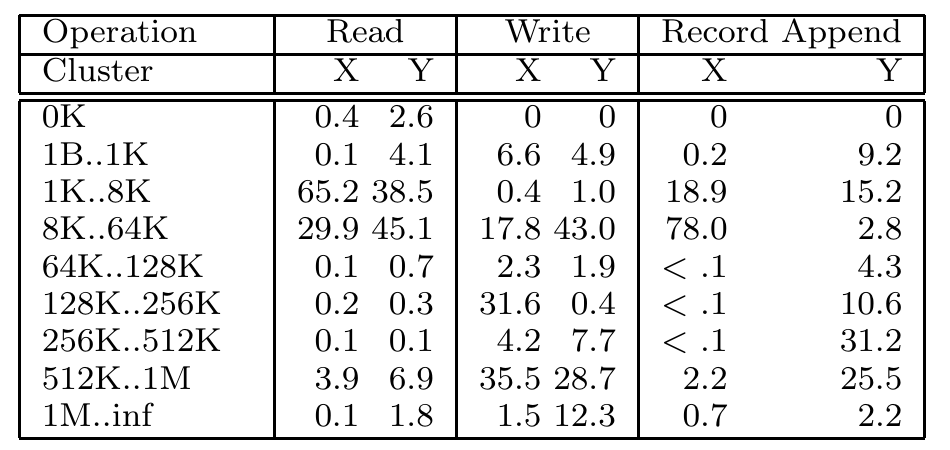
\includegraphics[width=0.95\columnwidth]{figures/original/gfs-table-4-operations-by-size.png}
  \refstepcounter{table}\label{tab:gfs-operations-by-size}

  {\small\textbf{Table 4.}按操作大小划分的操作占比(\%)}
\end{center}

\subsubsection{chunkserver访问负载}
Table4展示了按大小划分的操作分布。读取大小呈现双峰分布。
小读取(小于64KB)来自寻道密集型客户端，它们会在巨大文件中查找小片数据。
大读取(大于512KB)则来自对整个文件进行的长时间顺序读取。

集群Y中有相当数量的读取完全不返回数据。我们的应用，特别是生产系统中的应用，
常将文件用作生产者-消费者队列。生产者并发向文件追加数据，而消费者读取文件末尾。
当消费者的速度超过生产者时，偶尔会没有数据返回。集群X较少出现这种情况，因为它
通常用于短生命周期的数据分析任务，而非长生命周期的分布式应用。

写入大小同样呈现双峰分布。大写入(大于256KB)通常源于写入端进行了较大规模的缓冲。
缓冲数据较少、更频繁地进行checkpoint或同步、或者生成数据较少的写入端，会产生较小的写
入(小于64KB)。

对于\textbf{record append}，集群Y中大型\textbf{record append}所占比例远
高于集群X，因为使用集群Y的生产系统针对GFS进行了更积极的调优。

Table5展示了不同大小操作传输的数据总量。对于所有类型的操作，较大的操
作(大于256KB)通常占据大部分传输字节。由于随机寻道访问负载，小读取(小于64KB)也会
传输一部分虽小但不可忽略的读取数据。

\begin{center}
  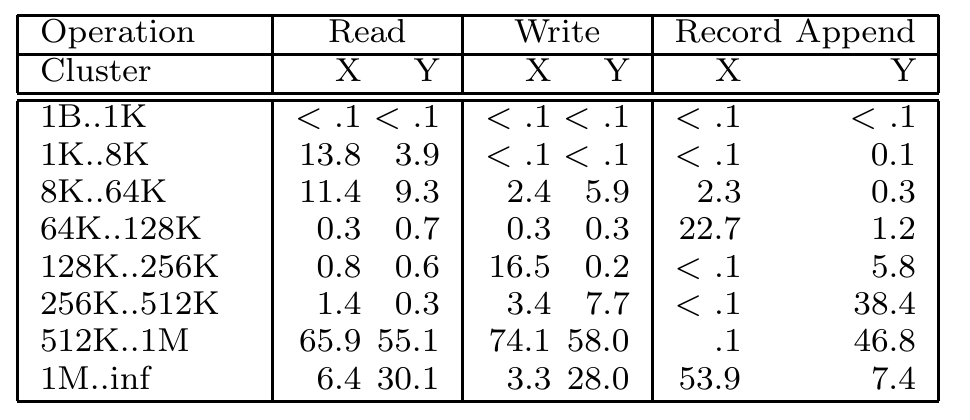
\includegraphics[width=0.95\columnwidth]{figures/original/gfs-table-5-bytes-transferred-by-operation-size.png}
  \refstepcounter{table}\label{tab:gfs-bytes-transferred-by-operation-size}

  {\small\textbf{Table 5.}按操作大小划分的传输字节数占比(\%)。对于读取操作，大小指
  实际读取并传输的数据量，而非请求的数据量。如果读取操作尝试读取超过文件末尾的数据，
  这两者可能不同；按照设计，这种情况在我们的访问负载中并不少见。}
\end{center}

\begin{center}
  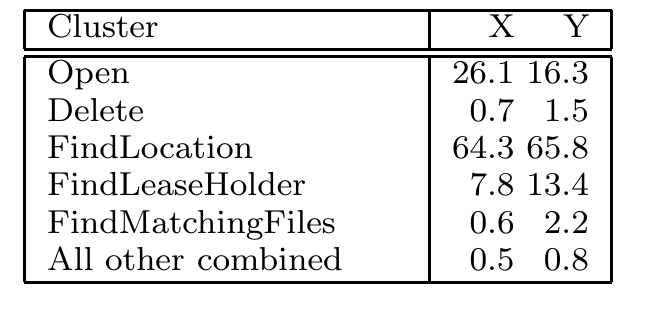
\includegraphics[width=0.82\columnwidth]{figures/original/gfs-table-6-master-requests-by-type.png}
  \refstepcounter{table}\label{tab:gfs-master-requests-by-type}

  {\small\textbf{Table 6.}按类型划分的master请求占比(\%)}
\end{center}

\subsubsection{append vs write}
\textbf{record append}被广泛使用，尤其是在我们的生产系统中。对于集群X，按传输字节
数计算，写入与\textbf{record append}的比例为10:1；按操作次数计算，比例为8:1。
对于用于生产系统的集群Y，这两个比例分别为3.7:1和2.5:1。此外，这些比例表明，两个集群
中的\textbf{record append}通常都比\textbf{write}更大。然而，对于集群X，在测量期间
\textbf{record append}的总体使用量相当低，因此结果很可能被一两个采用特
定缓冲区大小选择的应用所扭曲。

正如预期，我们的数据mutation访问负载以追加而非覆盖为主。我们测量了
primary replica上被覆盖的数据量。这近似于客户端有意覆盖此前写入的数据，而非追
加新数据的情形。对于集群X，覆盖操作占mutation字节数的不足0.0001\%，占
mutation操作数的不足0.0003\%。对于集群Y，这两个比例均为0.05\%。尽管
这一比例极小，但仍高于我们的预期。结果发现，大部分覆盖来自客户端因错误或超时而进行
的重试。它们本身并不属于访问负载，而是重试机制带来的结果。

\subsubsection{master访问负载}
Table 6展示了发送给master的请求按类型划分的构成。大多数请求用于读取时获取
chunk位置(\textbf{FindLocation})，以及进行数据mutation时获取lease持有者信
息(\textbf{FindLeaseLocker})。

集群X与Y的\textbf{Delete}请求数量显著不同，这是因为集群Y存储的生产数据集会定期重
新生成并由新版本替换。其中一部分差异还隐藏在\textbf{Open}请求数量的差异中，
因为文件的旧版本可能会在从头以写入模式打开时被隐式删除(按Unix的\textbf{open}术语，即\textbf{"w"}模式)。

\textbf{FindMatchingFiles}是一种支持\textbf{ls}及类似文件系统操作的模式匹配请求。
与其他发往master的请求不同，它可能需要处理命名空间中的很大一部分，因此开销可能较高。
集群Y更频繁地出现此类请求，因为自动化数据处理任务往往需要检查文件系统的某些部分，
以了解全局应用状态。相比之下，集群X中的应用受用户更明确的控制，通常会预先知道所有
所需文件的名称。
